\section{Arrizal Furqona Gifary (1174070)}
\subsection{Koordinat}
\begin{itemize}
	\item Sejarah Koordinat
Koordinat adalah suatu titik yang didapatkan dari hasil perpotongan dari garis latitude (lintang) dengan garis bujur (longitude) sehingga akan menunjukan lokasi pada suatu daerah. Umumnya koordinat dibedakan menjadi koordinat Geographic dan Universal Transver Mercator (UTM). 	
Menurut Heroditus (450-M) yaitu seorang ahli sejarah mengatakan bahwa geometri itu berasal dari Mesir. Rane Discartes (Matematikawan) adalah sesesorang yang memiliki ketertarikan di bidang geometri. Rane menemukan metode untuk menyajikan sebuah titik sebagai sebuah bilangan berpasangan dalam sebuah bidang datar. Bilangan-bilangan itu terletak pada dua garis yang saling tegak lurus antara satu dengan lainnya dan berpotongan di sebuah titik yaitu (0,0) yang dinamakan Origin, dan biasanya ditandai atau disimbold engan O (0,0). Bidang tersebut dinamakan bidang "Koordinat" atau yang biasa kita tau sebagai bidang kartesius.
	\item Sistem Koordinat Dua Dimensi
	\begin{enumerate}
	\item Sistem Koordinat Kartesius
	
Sistem koordinat ini digunakan untuk mendefinisikan jarak dari titik awal (0,0) kepada titik x yang disebut koordinat x (absis) dan titik y yang disebut koordinat y (ordinat) dari titik awal kita.
Untuk menggambarkan titik x dan y bisa dilihat pada(Gambar 1).
	\begin{figure}[H]
	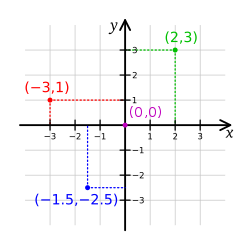
\includegraphics[width=4cm]{figures/Tugas1/1174070/kartesius.png}
	\centering
	\caption{Gambar 1}
\end{figure}
	
	\item Sistem Koordinat Polar

Sistem Koordinat Polar adalah sistem koordinat 2D yang titik bidangnya itu ditentukan dari jarak titik yang telah ditentukan dan suatu sudut dari arah yang sebelumnya telah ditentukan.

Titik yang sudah ditentukan disebut pole atau kutub, dan ray atau sinar dari kutub pada arah yang sudah ditentukan disebut dengan polar axis atau aksis polar. Jarak dari sebuah kutub disebut dengan radial coordinate atau radius dan sudutnya disebut dengan angular coordinate atau polar angle atau azimuth.

Contoh untuk Koordinat polar (Gambar 2).
	\begin{figure}[H]
	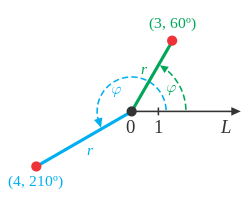
\includegraphics[width=4cm]{figures/Tugas1/1174070/polar.png}
	\centering
	\caption{Gambar 1}
\end{figure}
	\end{enumerate}
\end{itemize}
\subsection{Link}
https://youtu.be/pf1TGbKMJpU
\subsection{Plagiarism}
\begin{figure}[H]
	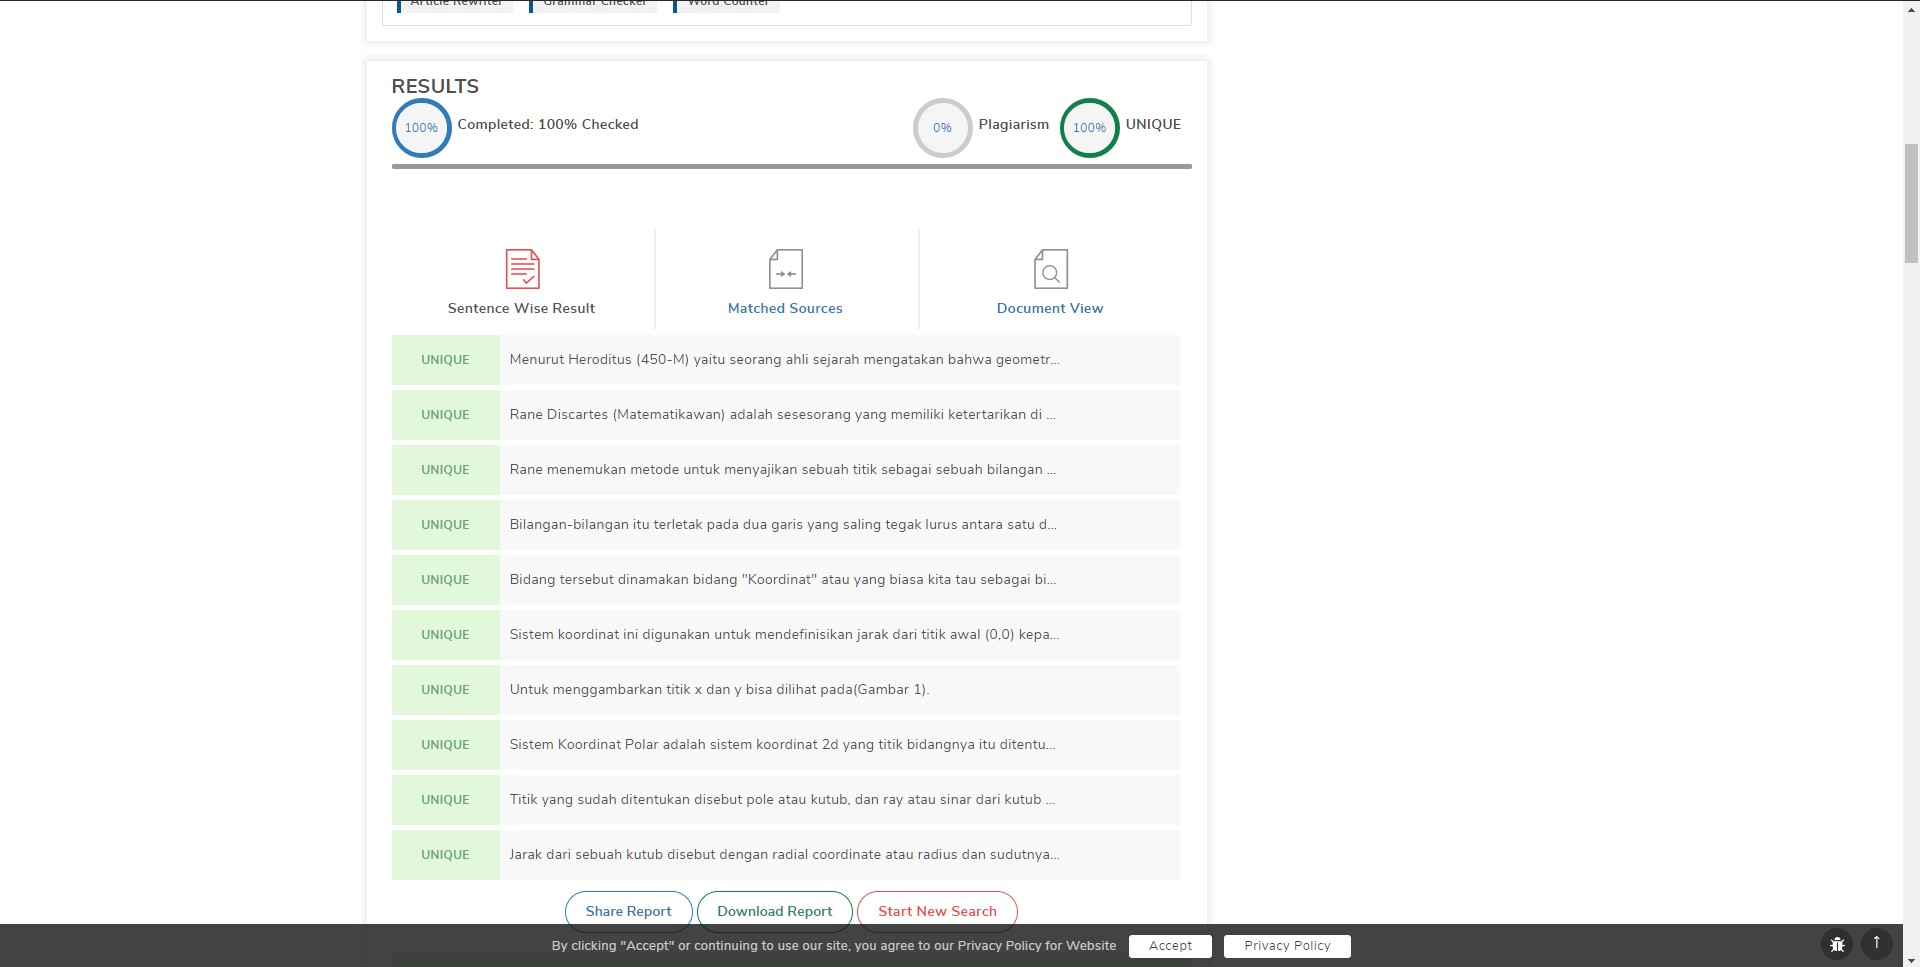
\includegraphics[width=4cm]{figures/Tugas1/1174070/plagiat.jpg}
	\centering
	\caption{Gambar Plagiat}
\end{figure}
